\documentclass{article}
\usepackage{tikz}
\usepackage{mathtools}
\usetikzlibrary{shapes, arrows, patterns, positioning}

\tikzstyle{startstop} rounded corners, minimum width=3cm, minimum height=1cm, text centered, draw=black, fill=gray!20]
\tikzstyle{process} minimum width=3cm, minimum height=1cm, text centered, draw=black, fill=blue!20]
\tikzstyle{decision} = [diamond, minimum width=3cm, minimum height=1cm, text centered, draw=black, fill=red!20]
\tikzstyle{arrow} = [thick,->,>=stealth]

\begin{document}

% \begin{center}
	% \resizebox{\textwidth}{!}{
	% 	\input{D:/Masterarbeit/tudothesis/tikz/LET.tex}
	% }
% \end{center}
	
\begin{figure}[h]
    \centering
    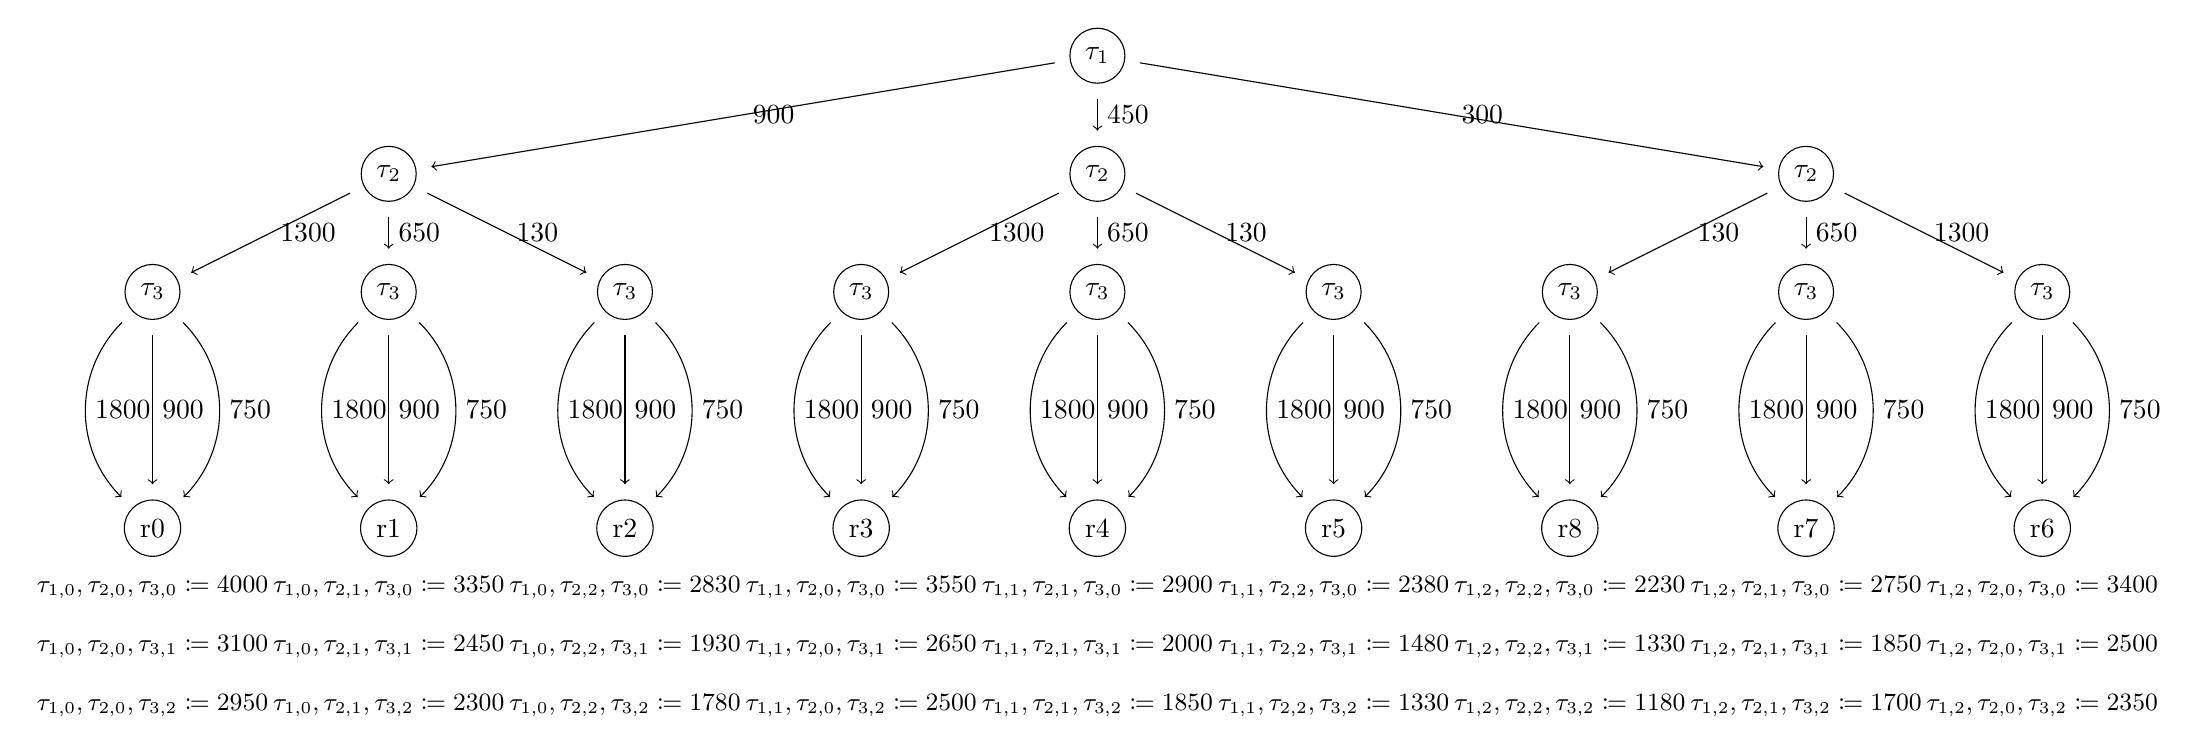
\begin{tikzpicture}
		
	\node[draw, circle, outer sep=2mm] (n10) at (0,0) {$\tau_1$};

	\node[draw, circle, outer sep=2mm] (n20) at (-9,-1.5) {$\tau_2$};
	\node[draw, circle, outer sep=2mm] (n21) at (0,-1.5) {$\tau_2$};
	\node[draw, circle, outer sep=2mm] (n22) at (9,-1.5) {$\tau_2$};

	\node[draw, circle, outer sep=2mm] (n30) at (-12,-3) {$\tau_3$};
	\node[draw, circle, outer sep=2mm] (n31) at (-9,-3) {$\tau_3$};
	\node[draw, circle, outer sep=2mm] (n32) at (-6,-3) {$\tau_3$};
	\node[draw, circle, outer sep=2mm] (n33) at (-3,-3) {$\tau_3$};
	\node[draw, circle, outer sep=2mm] (n34) at (0,-3) {$\tau_3$};
	\node[draw, circle, outer sep=2mm] (n35) at (3,-3) {$\tau_3$};
	\node[draw, circle, outer sep=2mm] (n36) at (12,-3) {$\tau_3$};
	\node[draw, circle, outer sep=2mm] (n37) at (9,-3) {$\tau_3$};
	\node[draw, circle, outer sep=2mm] (n38) at (6,-3) {$\tau_3$};

	\node[draw, circle, outer sep=2mm] (r0) at (-12,-6)	{r0};
	\node[draw, circle, outer sep=2mm] (r1) at (-9,	-6)	{r1};
	\node[draw, circle, outer sep=2mm] (r2) at (-6,	-6)	{r2};
	\node[draw, circle, outer sep=2mm] (r3) at (-3,	-6)	{r3};
	\node[draw, circle, outer sep=2mm] (r4) at (0,	-6)	{r4};
	\node[draw, circle, outer sep=2mm] (r5) at (3,	-6)	{r5};
	\node[draw, circle, outer sep=2mm] (r6) at (12,	-6)	{r6};
	\node[draw, circle, outer sep=2mm] (r7) at (9,	-6)	{r7};
	\node[draw, circle, outer sep=2mm] (r8) at (6,	-6)	{r8};

	\node[outer sep=0mm] (r01) at (-12,-6.75) {\small$\tau_{1,0},\tau_{2,0},\tau_{3,0}\coloneqq{}4000$};
	\node[outer sep=0mm] (r02) at (-12,-7.5)  {\small$\tau_{1,0},\tau_{2,0},\tau_{3,1}\coloneqq{}3100$};
	\node[outer sep=0mm] (r03) at (-12,-8.25) {\small$\tau_{1,0},\tau_{2,0},\tau_{3,2}\coloneqq{}2950$};
	\node[outer sep=0mm] (r11) at (-9, -6.75) {\small$\tau_{1,0},\tau_{2,1},\tau_{3,0}\coloneqq{}3350$};
	\node[outer sep=0mm] (r12) at (-9, -7.5)  {\small$\tau_{1,0},\tau_{2,1},\tau_{3,1}\coloneqq{}2450$};
	\node[outer sep=0mm] (r13) at (-9, -8.25) {\small$\tau_{1,0},\tau_{2,1},\tau_{3,2}\coloneqq{}2300$};
	\node[outer sep=0mm] (r21) at (-6, -6.75) {\small$\tau_{1,0},\tau_{2,2},\tau_{3,0}\coloneqq{}2830$};
	\node[outer sep=0mm] (r22) at (-6, -7.5)  {\small$\tau_{1,0},\tau_{2,2},\tau_{3,1}\coloneqq{}1930$};
	\node[outer sep=0mm] (r23) at (-6, -8.25) {\small$\tau_{1,0},\tau_{2,2},\tau_{3,2}\coloneqq{}1780$};
	\node[outer sep=0mm] (r31) at (-3, -6.75) {\small$\tau_{1,1},\tau_{2,0},\tau_{3,0}\coloneqq{}3550$};
	\node[outer sep=0mm] (r32) at (-3, -7.5)  {\small$\tau_{1,1},\tau_{2,0},\tau_{3,1}\coloneqq{}2650$};
	\node[outer sep=0mm] (r33) at (-3, -8.25) {\small$\tau_{1,1},\tau_{2,0},\tau_{3,2}\coloneqq{}2500$};
	\node[outer sep=0mm] (r41) at (0,  -6.75) {\small$\tau_{1,1},\tau_{2,1},\tau_{3,0}\coloneqq{}2900$};
	\node[outer sep=0mm] (r42) at (0,  -7.5)  {\small$\tau_{1,1},\tau_{2,1},\tau_{3,1}\coloneqq{}2000$};
	\node[outer sep=0mm] (r43) at (0,  -8.25) {\small$\tau_{1,1},\tau_{2,1},\tau_{3,2}\coloneqq{}1850$};
	\node[outer sep=0mm] (r51) at (3,  -6.75) {\small$\tau_{1,1},\tau_{2,2},\tau_{3,0}\coloneqq{}2380$};
	\node[outer sep=0mm] (r52) at (3,  -7.5)  {\small$\tau_{1,1},\tau_{2,2},\tau_{3,1}\coloneqq{}1480$};
	\node[outer sep=0mm] (r53) at (3,  -8.25) {\small$\tau_{1,1},\tau_{2,2},\tau_{3,2}\coloneqq{}1330$};
	\node[outer sep=0mm] (r61) at (12, -6.75) {\small$\tau_{1,2},\tau_{2,0},\tau_{3,0}\coloneqq{}3400$};
	\node[outer sep=0mm] (r62) at (12, -7.5)  {\small$\tau_{1,2},\tau_{2,0},\tau_{3,1}\coloneqq{}2500$};
	\node[outer sep=0mm] (r63) at (12, -8.25) {\small$\tau_{1,2},\tau_{2,0},\tau_{3,2}\coloneqq{}2350$};
	\node[outer sep=0mm] (r71) at (9,  -6.75) {\small$\tau_{1,2},\tau_{2,1},\tau_{3,0}\coloneqq{}2750$};
	\node[outer sep=0mm] (r72) at (9,  -7.5)  {\small$\tau_{1,2},\tau_{2,1},\tau_{3,1}\coloneqq{}1850$};
	\node[outer sep=0mm] (r73) at (9,  -8.25) {\small$\tau_{1,2},\tau_{2,1},\tau_{3,2}\coloneqq{}1700$};
	\node[outer sep=0mm] (r81) at (6,  -6.75) {\small$\tau_{1,2},\tau_{2,2},\tau_{3,0}\coloneqq{}2230$};
	\node[outer sep=0mm] (r82) at (6,  -7.5)  {\small$\tau_{1,2},\tau_{2,2},\tau_{3,1}\coloneqq{}1330$};
	\node[outer sep=0mm] (r83) at (6,  -8.25) {\small$\tau_{1,2},\tau_{2,2},\tau_{3,2}\coloneqq{}1180$};

	\draw[->] (n10) to node[midway, anchor=west] {900} (n20);
	\draw[->] (n10) to node[midway, anchor=west] {450} (n21);
	\draw[->] (n10) to node[midway, anchor=west] {300} (n22);

	\draw[->] (n20) to node[midway, anchor=west] {1300}(n30);
	\draw[->] (n20) to node[midway, anchor=west] {650} (n31);
	\draw[->] (n20) to node[midway, anchor=west] {130} (n32);
	\draw[->] (n21) to node[midway, anchor=west] {1300}(n33);
	\draw[->] (n21) to node[midway, anchor=west] {650} (n34);
	\draw[->] (n21) to node[midway, anchor=west] {130} (n35);
	\draw[->] (n22) to node[midway, anchor=west] {1300}(n36);
	\draw[->] (n22) to node[midway, anchor=west] {650} (n37);
	\draw[->] (n22) to node[midway, anchor=west] {130} (n38);

	\draw[->] (n30) to[in=135, out=225, edge label=1800](r0);
	\draw[->] (n30) to[in=90, out=270, edge label=900] (r0);
	\draw[->] (n30) to[in=45, out=315, edge label=750] (r0);
	\draw[->] (n31) to[in=135, out=225, edge label=1800](r1);
	\draw[->] (n31) to[in=90, out=270, edge label=900] (r1);
	\draw[->] (n31) to[in=45, out=315, edge label=750] (r1);
	\draw[->] (n32) to[in=135, out=225, edge label=1800](r2);
	\draw[->] (n32) to[in=90, out=270, edge label=900] (r2);
	\draw[->] (n32) to[in=45, out=315, edge label=750] (r2);
	\draw[->] (n33) to[in=135, out=225, edge label=1800](r3);
	\draw[->] (n33) to[in=90, out=270, edge label=900] (r3);
	\draw[->] (n33) to[in=45, out=315, edge label=750] (r3);
	\draw[->] (n34) to[in=135, out=225, edge label=1800](r4);
	\draw[->] (n34) to[in=90, out=270, edge label=900] (r4);
	\draw[->] (n34) to[in=45, out=315, edge label=750] (r4);
	\draw[->] (n35) to[in=135, out=225, edge label=1800](r5);
	\draw[->] (n35) to[in=90, out=270, edge label=900] (r5);
	\draw[->] (n35) to[in=45, out=315, edge label=750] (r5);
	\draw[->] (n36) to[in=135, out=225, edge label=1800](r6);
	\draw[->] (n36) to[in=90, out=270, edge label=900] (r6);
	\draw[->] (n36) to[in=45, out=315, edge label=750] (r6);
	\draw[->] (n37) to[in=135, out=225, edge label=1800](r7);
	\draw[->] (n37) to[in=90, out=270, edge label=900] (r7);
	\draw[->] (n37) to[in=45, out=315, edge label=750] (r7);
	\draw[->] (n38) to[in=135, out=225, edge label=1800](r8);
	\draw[->] (n38) to[in=90, out=270, edge label=900] (r8);
	\draw[->] (n38) to[in=45, out=315, edge label=750] (r8);



	\end{tikzpicture}
    \caption{Java Program Structure}\label{fig:java_structure}
\end{figure}
\end{document}


% \node[minimum width=3cm, minimum height=1cm] (table_node0) at (-12,-4.5){\small
% \begin{tabular}{|c|c|}
% 	\hline
% 	$\tau_{1,0},\tau_{2,0},\tau_{3,0}$ & 1 \\
% 	$\tau_{1,0},\tau_{2,0},\tau_{3,1}$ & 2 \\
% 	$\tau_{1,0},\tau_{2,0},\tau_{3,2}$ & 3 \\
% 	\hline
% \end{tabular}
% };
% \node[minimum width=3cm, minimum height=1cm] (table_node1) at (-9,-4.5){\small
% \begin{tabular}{|c|c|}
% 	\hline
% 	$\tau_{1,0},\tau_{2,1},\tau_{3,0}$ & 1 \\
% 	$\tau_{1,0},\tau_{2,1},\tau_{3,1}$ & 2 \\
% 	$\tau_{1,0},\tau_{2,1},\tau_{3,2}$ & 3 \\
% 	\hline
% \end{tabular}
% };
% \node[minimum width=3cm, minimum height=1cm] (table_node2) at (-6,-4.5){\small
% \begin{tabular}{|c|c|}
% 	\hline
% 	$\tau_{1,0},\tau_{2,2},\tau_{3,0}$ & 1 \\
% 	$\tau_{1,0},\tau_{2,2},\tau_{3,1}$ & 2 \\
% 	$\tau_{1,0},\tau_{2,2},\tau_{3,2}$ & 3 \\
% 	\hline
% \end{tabular}
% };

% \node[minimum width=3cm, minimum height=1cm] (table_node3) at (-3,-4.5){\small
% \begin{tabular}{|c|c|}
% 	\hline
% 	$\tau_{1,1},\tau_{2,0},\tau_{3,0}$ & 1 \\
% 	$\tau_{1,1},\tau_{2,0},\tau_{3,1}$ & 2 \\
% 	$\tau_{1,1},\tau_{2,0},\tau_{3,2}$ & 3 \\
% 	\hline
% \end{tabular}
% };
% \node[minimum width=3cm, minimum height=1cm] (table_node4) at (0,-4.5){\small
% \begin{tabular}{|c|c|}
% 	\hline
% 	$\tau_{1,1},\tau_{2,1},\tau_{3,0}$ & 1 \\
% 	$\tau_{1,1},\tau_{2,1},\tau_{3,1}$ & 2 \\
% 	$\tau_{1,1},\tau_{2,1},\tau_{3,2}$ & 3 \\
% 	\hline
% \end{tabular}
% };
% \node[minimum width=3cm, minimum height=1cm] (table_node5) at (3,-4.5){\small
% \begin{tabular}{|c|c|}
% 	\hline
% 	$\tau_{1,1},\tau_{2,2},\tau_{3,0}$ & 1 \\
% 	$\tau_{1,1},\tau_{2,2},\tau_{3,1}$ & 2 \\
% 	$\tau_{1,1},\tau_{2,2},\tau_{3,2}$ & 3 \\
% 	\hline
% \end{tabular}
% };
% \node[minimum width=3cm, minimum height=1cm] (table_node6) at (12,-4.5){\small
% \begin{tabular}{|c|c|}
% 	\hline
% 	$\tau_{1,2},\tau_{2,0},\tau_{3,0}$ & 1 \\
% 	$\tau_{1,2},\tau_{2,0},\tau_{3,1}$ & 2 \\
% 	$\tau_{1,2},\tau_{2,0},\tau_{3,2}$ & 3 \\
% 	\hline
% \end{tabular}
% };
% \node[minimum width=3cm, minimum height=1cm] (table_node7) at (9,-4.5){\small
% \begin{tabular}{|c|c|}
% 	\hline
% 	$\tau_{1,2},\tau_{2,1},\tau_{3,0}$ & 1 \\
% 	$\tau_{1,2},\tau_{2,1},\tau_{3,1}$ & 2 \\
% 	$\tau_{1,2},\tau_{2,1},\tau_{3,2}$ & 3 \\
% 	\hline
% \end{tabular}
% };
% \node[minimum width=3cm, minimum height=1cm] (table_node8) at (6,-4.5){\small
% \begin{tabular}{|c|c|}
% 	\hline
% 	$\tau_{1,2},\tau_{2,2},\tau_{3,0}$ & 1 \\
% 	$\tau_{1,2},\tau_{2,2},\tau_{3,1}$ & 2 \\
% 	$\tau_{1,2},\tau_{2,2},\tau_{3,2}$ & 3 \\
% 	\hline
% \end{tabular}
% };
